% generated by Plantuml 1.2022.7       
\definecolor{plantucolor0000}{RGB}{241,241,241}
\definecolor{plantucolor0001}{RGB}{24,24,24}
\definecolor{plantucolor0002}{RGB}{173,209,178}
\definecolor{plantucolor0003}{RGB}{0,0,0}
\definecolor{plantucolor0004}{RGB}{200,41,48}
\definecolor{plantucolor0005}{RGB}{242,77,92}
\definecolor{plantucolor0006}{RGB}{132,190,132}
\definecolor{plantucolor0007}{RGB}{3,128,72}
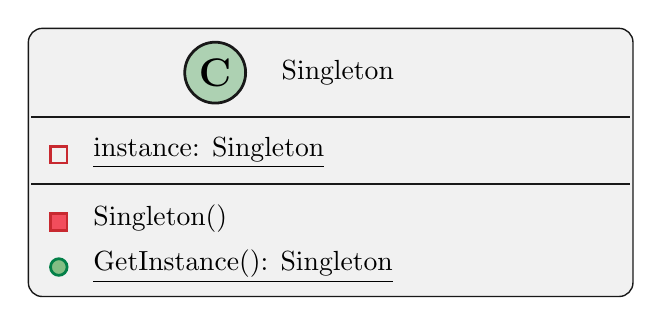
\begin{tikzpicture}[yscale=-1
,pstyle2/.style={color=plantucolor0001,line width=0.5pt}
]
\draw[color=plantucolor0001,fill=plantucolor0000,line width=0.5pt] (7pt,12pt) arc (180:270:5pt) -- (12pt,7pt) -- (220.4706pt,7pt) arc (270:360:5pt) -- (225.4706pt,12pt) -- (225.4706pt,98.8906pt) arc (0:90:5pt) -- (220.4706pt,103.8906pt) -- (12pt,103.8906pt) arc (90:180:5pt) -- (7pt,98.8906pt) -- cycle;
\draw[color=plantucolor0001,fill=plantucolor0002,line width=1.0pt] (74.5065pt,23pt) ellipse (11pt and 11pt);
\node at (74.5065pt,23pt)[]{\textbf{\Large C}};
\node at (95.0065pt,14.8516pt)[below right,color=black]{Singleton};
\draw[pstyle2] (8pt,39pt) -- (224.4706pt,39pt);
\draw[color=plantucolor0004,line width=1.0pt] (15pt,49.6484pt) rectangle (21pt,55.6484pt);
\node at (27pt,43pt)[below right,color=black]{\underline{instance: Singleton}};
\draw[pstyle2] (8pt,63.2969pt) -- (224.4706pt,63.2969pt);
\draw[color=plantucolor0004,fill=plantucolor0005,line width=1.0pt] (15pt,73.9453pt) rectangle (21pt,79.9453pt);
\node at (27pt,67.2969pt)[below right,color=black]{Singleton()};
\draw[color=plantucolor0007,fill=plantucolor0006,line width=1.0pt] (18pt,93.2422pt) ellipse (3pt and 3pt);
\node at (27pt,83.5938pt)[below right,color=black]{\underline{GetInstance(): Singleton}};
\end{tikzpicture}
